% Portrait option: replace the old figure and its three explanatory paragraphs.
% Compile from workshop_v2/论文/. Keep exactly one fig:roadmap.
% Width is 160 mm in the current paper; same-width gain is only 1.33%.
\begin{figure}[htbp]\centering
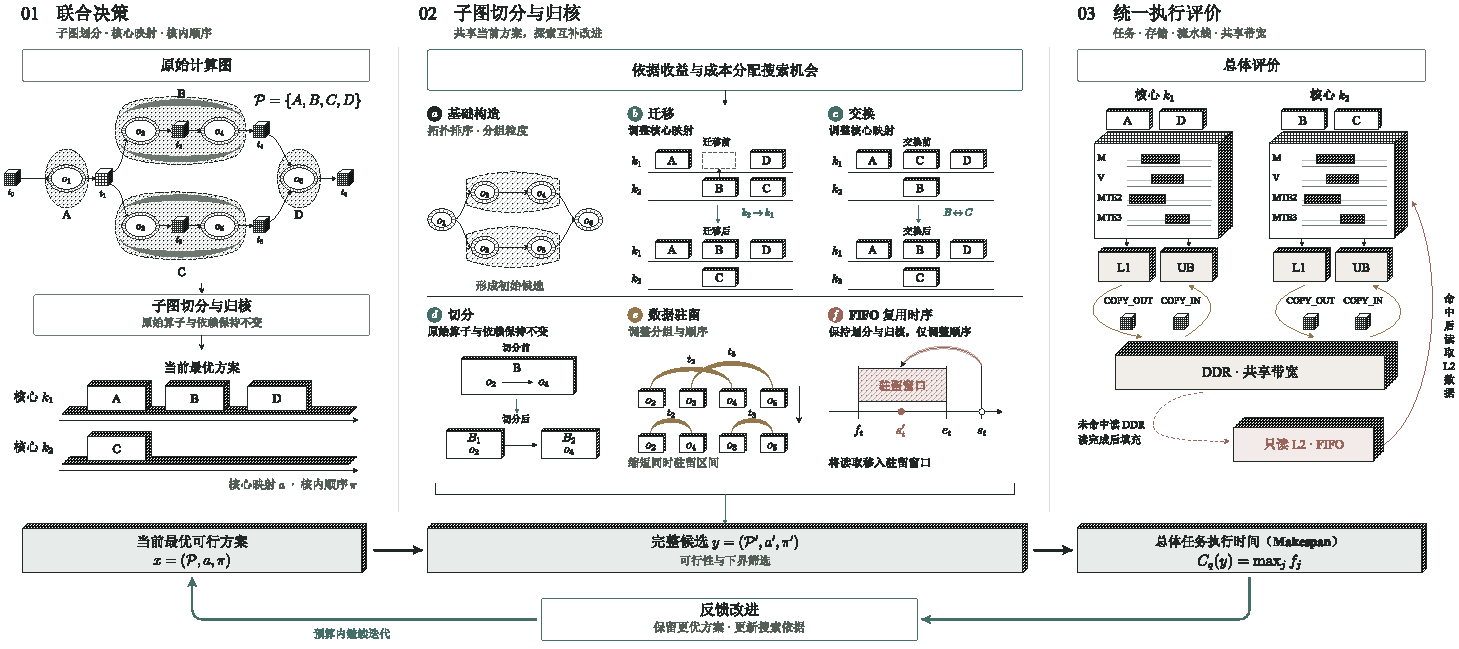
\includegraphics[width=\textwidth]{../../../../paper_a_figures/engraved_workflow/ink_v12/exports/workflow_qinglu_v12.pdf}
\caption{联合决策、子图切分与归核及统一执行评价}\label{fig:roadmap}
\end{figure}

如图~\ref{fig:roadmap} 所示，首先将子图划分、核心映射与核内顺序组成完整方案，再围绕当前方案，通过基础构造、迁移、交换、切分、数据驻留和FIFO复用时序调整生成候选。问题一采用（a）—（d），问题二增加（e），问题三再增加（f）。候选经可行性与下界筛选后，按任务、存储、流水线及共享带宽约束统一评价，优先保留总体任务执行时间较短、周期相同时总额外数据搬运量较少的方案，并根据收益与成本分配后续搜索机会。第三问的\texttt{COPY\_IN}在发射时查询只读L2，命中由L2服务，未命中则读取DDR，读完成后按容量与FIFO规则尝试填充；\texttt{COPY\_OUT}仍写入DDR。上述过程在预算内迭代，最终输出当前最优可行方案，并固定第三问方案进行无L2与有L2的配对评价。
